\section{Results}
This is the data analysis plan for this study. This section also includes figures from my first year project that can outline the current direction of my thesis. 
\begin{itemize}
	\item Once data collection is complete, the data will be cleaned and processed using standard protocol. Data will be processed in EEGLab via MATLAB. Difference waveforms will be calculated by subtracting the conflict conditions (SCFI, SIFC and SIFI) from SCFC.
	\item These difference waveforms will be used to extract pure conflict processing activity and remove other irrelevant mental processes. 
	\item Planned statistical analyses include repeated-measures ANOVA for the different variables including LRP, P3 and reaction time. Additionally, linear mixed models will be used to test the interactions between P3 and LRP across different conflicts and conditions. Analyses will also incorporate AUDIT and I-8 scores to examine differences between heavy drinkers and highly impulsive individuals from healthy controls. 
	\item The main analysis may simplify by focusing on Equal condition and SIFI, but exploratory analyses (TBD) will determine how AUDIT and I-8 scores relate to the different conflicts and conditions. 
	\item The base for my thesis will be an expanded version of the theoretical model of my FYP.
\end{itemize}
\begin{figure}[ht!]
\centering
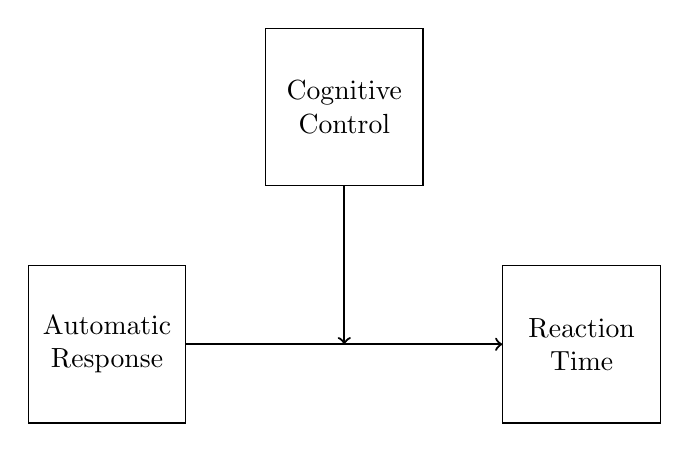
\begin{tikzpicture}
\usetikzlibrary{positioning}
\node [draw, align=center, minimum width=2cm, minimum height=2cm, inner sep=2pt] (CC) at (0,0) {Cognitive\\ Control};
\node [draw, align=center, minimum width=2cm, minimum height=2cm, inner sep=2pt] (RT) [below right=of CC] {Reaction\\ Time};
\node [draw, align=center, minimum width=2cm, minimum height=2cm, inner sep=2pt] (LRP) [below left=of CC] {Automatic \\ Response};
\path[->,thick](LRP)edge(RT);
\path (LRP) -- (RT) coordinate[midway] (midpoint);
\draw [->,thick](CC) -- (midpoint);
\end{tikzpicture}
\caption{Here is the theoretical model that my thesis will be expanding.}
\label{fig:FYP} 
\end{figure}

\begin{figure}[htbp] 
\centering
\includegraphics[width=0.8\textwidth]{totalfigs_copy}
\caption{Here are some figures for my P3b and LRP data}
\label{fig:ERPs}
\end{figure}

\begin{table}[h!]
\centering
\caption{\label{tab:RTmeans}Reaction times for different Simon-Flanker conflict and PC effect conditons.}
\begin{tabular}{l l c c c}
 \toprule
                          &              & \multicolumn{3}{c}{Condition, seconds}\\
  \cmidrule{3-5}
                          &              & {Equal}           & {Incongruent}           & {Congruent}\\
  \cmidrule{3-5}
  \multirow{ 4}{*}{Conflict} & SCFC &     0.595    &      0.603     &      0.585     \\
                          & SCFI      &     0.654      &      0.671     &      0.639   \\
                          & SIFC     &     0.624     &     0.621     &     0.641     \\
                          & SIFI     &      0.712    &     0.703     &     0.716    \\
  \bottomrule
 \end{tabular}
\end{table}
